% Kopfzeile beim Kapitelanfang:
\fancypagestyle{plain}{
%Kopfzeile links bzw. innen
\fancyhead[L]{\Large Vorlesung 26 (23.01.2013)}
%Kopfzeile rechts bzw. außen
\fancyhead[R]{}}
%Kopfzeile links bzw. innen
\fancyhead[L]{\Large Vorlesung 26 (23.01.2014)}
%Kopfzeile rechts bzw. außen
\fancyhead[R]{}
% **************************************************
\subsection*{Beweis}
\en{
\item Seien $(\varphi), (\psi) \subseteq T[a,b]$ mit $\|f-\varphi_n\| \to 0, \|g-\psi_n\| \to 0$\\
$\Ra \|f+g-\underbrace{\varphi_n+\psi_n)}_{\in T[a,b]}\| \underset{\text{Dreiecksungl.}}{\le} \|f-\varphi_n\|+\|g-\psi_n\| \to 0$\\
$\Ra \int_a^b (f+g) dx = \lim_{n \to \infty} \int_a^b (\varphi_n+\psi_n) dx \underset{\text{\ref{14.2}}}{=} \lim_{n \to \infty} \left(\int_a^b \varphi_n dx + \int_a^b \psi_n dx\right) = \int_a^b f dx + \int_a^b g dx$
}
Rest analog. \qed\nl
Seien $a < b < c, f \in R[a,c] \Ra f$ eigenschränkt auf $[a,b]$ und $[b,c]$ ist Regelfunktion\\
und $\int_a^c f dx = \int_a^b fdx + \int_b^c f dx$ (mit Approx. durch Treppenf.)\nl
Konvention: $a < b, f \in R[a,b]$:
$$\int_b^a f dx := -\int_a^b fdx, \int_a^a fdx := 0$$

\section{Satz: Charakterisierung von Regelfunktionen}\label{14.6}
$f: [a,b] \to \R$ ist Regelfunktion $\Lra \forall x_0 \in (a,b] \exists \lim_{x \uparrow x_0} f(x) \in \R \ \wedge \ \forall x_0 \in [a,b) \exists \lim_{x \downarrow x_0} f(x) \in \R$\nl
\begin{tikzpicture}
\draw (-1.5,0) node[below] {$a$} --(1.5,0) node[below] {$b$};
\draw[dashed] (-1.5,0.5)--(-1.5,0) (1.5,3)--(1.5,0);
\draw[color=blue] (-1.5,0.5) node {$\bullet$} --(-0.5,1) node {$\circ$} (-0.5,2) node {$\bullet$} --(0.5,1) node {$\circ$} (0.5,2) node {$\bullet$} (0.5,2.5) node{$\circ$} --(1.5,3) node{$\bullet$};
\end{tikzpicture}

\section{Korollar}\label{14.7}
\en{
\item Jede stetige Funktion auf $[a,b]$ ist Regelfunktion
\item Jede monotone Funktion auf $[a,b]$ ist Regelfunktion
}

\subsection*{Beweis von (2)}
Sei $x_0 \in (a,b], f$ monoton wachsend.\\
Behauptung: $\lim_{x \uparrow x_0} f(x) = \sup_{x \in [a,x_0)} f(x) =: s \in \R$ (existiert, da $f$ beschränkt)\\
Sei $\eps > 0 \Ra \exists \xi \in [a,x_0): s-\eps < f(\xi) \le s$\\
$f$ mon. wachsend $\Ra \forall x \in [\xi,x_0): s-\eps < f(x) \le s$\\
$\underset{\text{Kor. \ref{9.12}}}{\Ra}$ Behauptung. \qed\nl
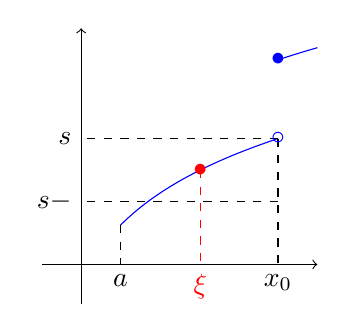
\begin{tikzpicture}
\draw[->] (-0.5,0)--(3,0);
\draw[->] (0,-0.5)--(0,3);
\draw[dashed] (0.5,0.5)--(0.5,0) node[below] {$a$} (2.5,1.598612288)--(2.5,0) node[below] {$x_0$} (2.5,1.598612288)--(0,1.598612288) node[left] {$s$} (2.5,0.8)--(0,0.8) node[left] {$s-\eps$};
\draw[color=blue,domain=0.5:2.48] plot (\x, {ln(\x+0.5)+0.5}) (2.5,1.598612288) node {$\circ$};
\draw[color=blue,domain=2.5:3] plot (\x, {ln(\x+0.5)+1.5}) (2.5,2.598612288) node {$\bullet$};
\draw[color=red,dashed] (1.51375270747048,1.2) node {$\bullet$} --(1.51375270747048,0) node[below] {$\xi$};
\end{tikzpicture}

\newpage

\subsection*{Gegenbeispiele}
\en{
\item $f(x) = \left\{\begin{array}{l l} \frac{1}{x}, & x \in (0,1] \\ 1, & x=0 \end{array}\right. \text{ auf } [0,1]$\nl
\begin{tikzpicture}
\draw[->] (-0.5,0)--(1.5,0);
\draw[->] (0,-0.5)--(0,2);
\draw[color=blue, domain=0.5:1] plot (\x, {1/\x}) (1,1) node {$\bullet$} node[above] {$f$};
\draw[dashed] (1,1)--(1,0) node[below] {$1$} (1,1)--(0,1) node[left] {$1$};
\end{tikzpicture}\nl
Keine Regelfunktion: $\lim_{x \downarrow 0} f(x) = +\infty$
\item Dirichletsche Sprungfunktion:\nl
$f(x) = \left\{\begin{array}{l l} 1, & x \in \Q \\ 0, & x \in \R \setminus \Q \end{array}\right.$\\
ist auf keinem $[a,b] \subseteq \R$ Regelfunktion (die Limiten existieren nirgends)
}
Weitere Konsequenz von \ref{14.6}: $f,g \in R[a,b] \Ra f \cdot g \in R[a,b]$

\section{Mittelwertsatz der Integralrechnung}\label{14.8}
Sei $f: [a,b] \to \R$ stetig, $p: [a,b] \to \R$ Regelfunktion, $p \ge 0$
$$\Ra \exists \xi \in [a,b]: \int_a^b f(x) p(x) dx = f(\xi) \cdot \int_a^b p(x) dx$$
Für $p=1$: $\int_a^b f dx = f(\xi) \cdot (b-a)$

\subsection*{Beweis}
$m := \min_{[a,b]} f, M := \max_{[a,b]} f$ (Satz von Minimum/Maximum, \ref{9.20})\\
$\Ra m \cdot p \le f \cdot p \le M \cdot p$ auf $[a,b]$\\
$\Ra m \cdot \int_a^b p dx \le \int_a^b fp dx \le M \cdot \int_a^b p dx$\\
$\Ra \int_a^b fp dx = c \cdot \int_a^b p dx$ mit $c \in [m,M]$\\
Zwischenwertsatz (\ref{9.18}) $\Ra \exists \xi \in [a,b]: c=f(\xi)$ \qed

\phantomsection
\addcontentsline{toc}{chapter}{Integration und Differentiation}
\chapter*{Integration und Differentiation}
\section{Definition: Stammfunktion}\label{14.9}
Sei $f: [a,b] \to \R$ eine Funktion.\\
$F: [a,b] \to \R$ heißt \underline{Stammfunktion} von $f :\Lra F$ differenzierbar mit $F'=f$ auf $[a,b]$

\section{Lemma}\label{14.10}
$F, G$ Stammfunktikonen von $f \Ra F-G=$ konstant

\subsection*{Beweis}
$(F-G)'=0$ auf $[a,b] \underset{\text{\ref{11.13}}}{\Ra}$ Behauptung. \qed

\section{Hauptsatz der Differential- und Integralrechnung (HDI)}\label{14.11}
Sei $f: [a,b] \to \R$ stetig, $x_0 \in [a,b]$\\
\fbox{$F(x) := \int_{x_0}^x f(t) dt$}, $x \in [a,b] \Ra$
\en{
\item $F$ ist Stammfunktion von $f$, das heißt $F$ differenzierbar auf $[a,b]$ mit $F'=f$
\item Ist $G: [a,b] \to \R$ beliebige Stammfunktion von $f \Ra$ \fbox{$\int_a^b f(t) dt = G(b)-G(a) =: G \mid_a^b$}
}

\subsection*{Beweis}
\en{
\item Sei $x \in [a,b], x+h \in [a,b]$\\
$\Ra \frac{F(x+h)-F(x)}{h} = \frac{1}{h} \left(\int_{x_0}^{x+h} f dt - \int_{x_0}^x f dt\right) = \frac{1}{h} \cdot \int_x^{x+h} 1 \cdot f(t) dt$\\
$\underset{\text{\ref{14.8}}}{=} \frac{1}{h} \cdot f(\xi) \cdot \underbrace{\int_x^{x+h} 1 dt}_{=h}, \xi \in [x,x+h]$\\
$=f(\xi)$\\
$h \to 0 \Ra x+h \to x \Ra \xi \to x \underset{f \text{ stetig}}{\Ra} f(\xi) \to f(x)$ für $h \to 0$\\
$F$ differenzierbar in $x, F'(x)=f(x)$
\item $F(x) := \int_a^x f(t) dt \Ra F,G$ Stammfunktionen von $f$\\
$\underset{\text{\ref{14.10}}}{\Ra} F-G=$ konst. $\Ra \int_a^b f(t) dt = F(b) - \underbrace{F(a)}_{=0} = G(b)-G(a)$
}\qed

\newpage

\subsection*{Bezeichnung}
Sei $f \in R[a,b]$. Für die Aussage "`$F$ ist Stammfunktion von $f$"' schreibt man:\\
$\int f(x) dx = F(x)$\\
"'\underline{Unbestimmtes Integral}"' von $f$ (eindeutig nur bis auf additive Konstante)

\section{Beispiele}
\enk{
\item $s \in \R \setminus \{-1\}$\\
$\Ra \int_a^b x^s dx = \frac{1}{s+1} x^{s+1} \arrowvert_a^b$\\
Dabei $[a,b] \subseteq \R$ fällt $s \in \Z, 0 \notin [a,b]$ falls $z \in \Z, s < 0$\\
(über die Definitionslücke darf nicht hinaus integriert werden!)\nl
Falls $s \in \R \setminus \Z$: $x^s = e^{s \ln x}$für $x > 0$, Also $a,b > 0$\\
kurz: $\int x^s dx = \frac{1}{s+1} x^{s+1}$ ($s \neq -1$)
\item $\int_a^b \frac{1}{x} dx = \left\{\begin{array}{l l} \ln x \arrowvert_a^b & a,b > 0 \\ \ln(-x) \arrowvert_a^b & a,b < 0 \end{array}\right.$\\
kurz: $\int \frac{1}{x} dx = \ln |x|$
\item $\int e^{cx} dx = \frac{1}{c} e^{cx}$ für $c \in \R \setminus \{0\}$
\item $\int \cos(x) dx = \sin(x)$, $\int \sin(x) dx = -\cos(x)$
\item $\int \frac{dx}{\sqrt{1-x^2}} = \arcsin(x)$ auf $(-1,1)$
\item $\int \frac{dx}{1+x^2} = \arctan(x)$ auf $\R$
\item $\int \frac{dx}{x^2-1}=$?\\
$R(x) = \frac{1}{x^2-1}=\frac{1}{(x-1)(x+1)}$ zwei verschiedene Nullstellen im Nenner\\
Partialbruchzerlegung: $R(x)=\frac{a}{x-1}+\frac{b}{x+1}$ mit\\
$a=(x-1)R(x) \arrowvert_{x=1} = \frac{1}{2}$, $b=(x+1)R(x) \arrowvert_{x=-1} = -\frac{1}{2}$\\
$\Ra \frac{1}{x^2-1}=\frac{1}{2} \left(\frac{1}{x-1}-\frac{1}{x+1}\right)$\\
$\Ra \int \frac{dx}{x^2-1} = \frac{1}{2} \int \frac{dx}{x-1} - \frac{1}{2} \int \frac{dx}{x+1} = \frac{1}{2} (\ln|x-1|-\ln|x+1|)=\frac{1}{2} \ln \left|\frac{x-1}{x+1}\right|$ (auf $\R \setminus\{\pm 1\}$)
}

\phantomsection
\addcontentsline{toc}{chapter}{Integrationstechniken}
\chapter*{Integrationstechniken}
\section{Partielle Integration}\label{14.13}
$f,g: [a,b] \to \R$ stetig differenzierbar $\Ra$
$$\int_a^b f \cdot g' dx = f \cdot g \arrowvert_a^b - \int_a^b f' \cdot g dx$$
bzw.
$$\int f \cdot g' dx = f \cdot g - \int f' \cdot g dx$$

\subsection*{Beweis}
$$(fg) \arrowvert_a^b \underset{\text{HDI (\ref{14.11})}}{=} \int_a^b (fg)' dx = \int_a^b f' g dx + \int_a^b fg' dx$$

\subsection*{Beispiele}
\enk{
\item $\int_0^1 \underset{f}{x} \cdot \underset{g'}{e^x} dx = \underbrace{x \cdot e^x \arrowvert_0^1}_{e} - \int_0^1 e^x dx = e - e^x \arrowvert_0^1 = 1$
\item $\int \ln(x) dx = \int \underset{g'}{1} \cdot \underset{f}{\ln(x)} dx = x \cdot \ln(x) - \int x \cdot \frac{1}{x} dx = x \cdot \ln(x) - x = x \cdot (\ln(x)-1)$
}

\section{Substitutionsregel}\label{14.14}
Sei $f: I \to \R$ stetig ($I$ Intervall), und $\varphi: [a,b] \to I$ stetig differenzierbar mit $\varphi([a,b]) \subseteq I$\\
$\Ra \int_a^b f(\varphi(t)) \cdot \varphi'(t) dt = \int_{\varphi(a)}^{\varphi(b)} f(x) dx$